\documentclass[11pt,oneside]{article}
\usepackage[T1]{fontenc}
\usepackage[utf8]{inputenc}
%\DeclareUnicodeCharacter{00A0}{ }
\usepackage[adobe-utopia]{mathdesign}

\usepackage{amsmath}
\usepackage[francais]{babel}
\usepackage[dvips]{graphicx}
%\usepackage{here}
\usepackage{framed}
\usepackage[normalem]{ulem}
\usepackage{fancyhdr}
\usepackage{titlesec}
\usepackage{vmargin}

\usepackage{amsmath}
\usepackage{ifthen}
\usepackage{multirow}
\usepackage{multicol} % Portions de texte en colonnes

%\usepackage{xltxtra} % Logo XeLaTeX
%\usepackage{pst-solides3d}
\usepackage{color}
%\usepackage{colortbl}
\usepackage{titletoc} % Pour la mise en forme de la table des matières

%\usepackage[crop=off]{auto-pst-pdf}
%\usepackage{bclogo}


%\usepackage{longtable}
%\usepackage{flafter}%floatants après la référence
%\usepackage{pst-solides3d}
%\usepackage{pstricks}
%\usepackage{minitoc}
%\setcounter{minitocdepth}{4}
%\usepackage{draftcopy}% "Brouillon"
%\usepackage{floatflt}
%\usepackage{psfrag}
%\usepackage{listings} % Permet d'insérer du code de programmation
%\usepackage{lmodern}
%\usepackage[adobe-utopia,uppercase=upright,greeklowercase=upright]{mathdesign}
%\usepackage{minionpro}
%\usepackage{pifont}
%\usepackage{amssymb}
%\usepackage[francais]{varioref}

\setmarginsrb{1.5cm}{1cm}{1cm}{1.5cm}{1cm}{1cm}{1cm}{1cm}

\definecolor{gris25}{gray}{0.75}
\definecolor{bleu}{RGB}{18,33,98}
\definecolor{bleuf}{RGB}{42,94,171}
\definecolor{bleuc}{RGB}{231,239,247}
\definecolor{rougef}{RGB}{185,18,27}
\definecolor{rougec}{RGB}{255,230,231}
\definecolor{vertf}{RGB}{103,126,82}
\definecolor{vertc}{RGB}{220,255,191}
\definecolor{violetf}{RGB}{112,48,160}
\definecolor{violetc}{RGB}{230,224,236}
\definecolor{jaunec}{RGB}{220,255,191}

\usepackage[%
    pdftitle={TD Conception},
    pdfauthor={Xavier Pessoles},
    colorlinks=true,
    linkcolor=blue,
    citecolor=magenta]{hyperref}



% \makeatletter \let\ps@plain\ps@empty \makeatother
%% DEBUT DU DOCUMENT
%% =================
\sloppy
\hyphenpenalty 10000

\newcommand{\Pointilles}[1][3]{%
\multido{}{#1}{\makebox[\linewidth]{\dotfill}\\[\parskip]
}}


\begin{document}


\newboolean{prof}
\setboolean{prof}{false}
%------------- En tetes et Pieds de Pages ------------
\pagestyle{fancy}
\renewcommand{\headrulewidth}{0pt}

\fancyhead{}
\fancyhead[L]{%
\begin{minipage}[c]{1.6cm}

\includegraphics[width=2cm]{png/logo_ptsi.png}%
\end{minipage}
\rule{2cm}{.5pt}
}

\fancyhead[C]{\rule{11cm}{.5pt}}

\fancyhead[R]{%
\begin{minipage}[c]{3cm}
\begin{flushright}
\footnotesize{\textit{\textsf{Sciences Industrielles\\ pour l'Ingénieur}}}%
\end{flushright}
\end{minipage}
}

\renewcommand{\footrulewidth}{0.2pt}

\fancyfoot[C]{\footnotesize{\bfseries \thepage}}
\fancyfoot[L]{\footnotesize{2011 -- 2012} \\ X. \textsc{Pessoles}}
\ifthenelse{\boolean{prof}}{%
\fancyfoot[R]{\footnotesize{TD -- CI 5 : Communication technique -- P}}
}{%
\fancyfoot[R]{\footnotesize{TD -- CI 5 : Communication technique}}
}


%\begin{center}
%\textit{Centre d'intérêt}
%\end{center}


\begin{center}
 \huge\textsc{CI 4 -- Conception des mécanismes}
\end{center}

\begin{center}
 \LARGE\textsc{Représentation des éléments filetés}
\end{center}

\begin{center}
 \large\textsc{TD 1 -- Emporte pièce}
\end{center}
\vspace{.5cm}


\begin{minipage}[c]{.3\linewidth}
\begin{center}
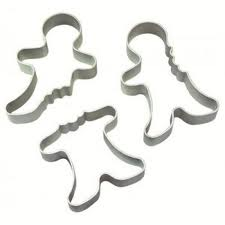
\includegraphics[height=3cm]{png/piece1}

\textit{Emporte pièce utilisé en pâtisserie}
\end{center}
\end{minipage}\hfill
\begin{minipage}[c]{.3\linewidth}
\begin{center}
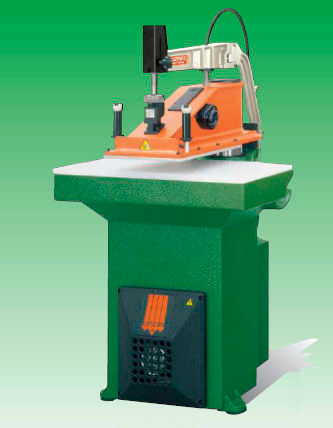
\includegraphics[height=3cm]{png/piece2}

\textit{Emporte pièce semi automatisé}
\end{center}
\end{minipage}\hfill
\begin{minipage}[c]{.3\linewidth}
\begin{center}
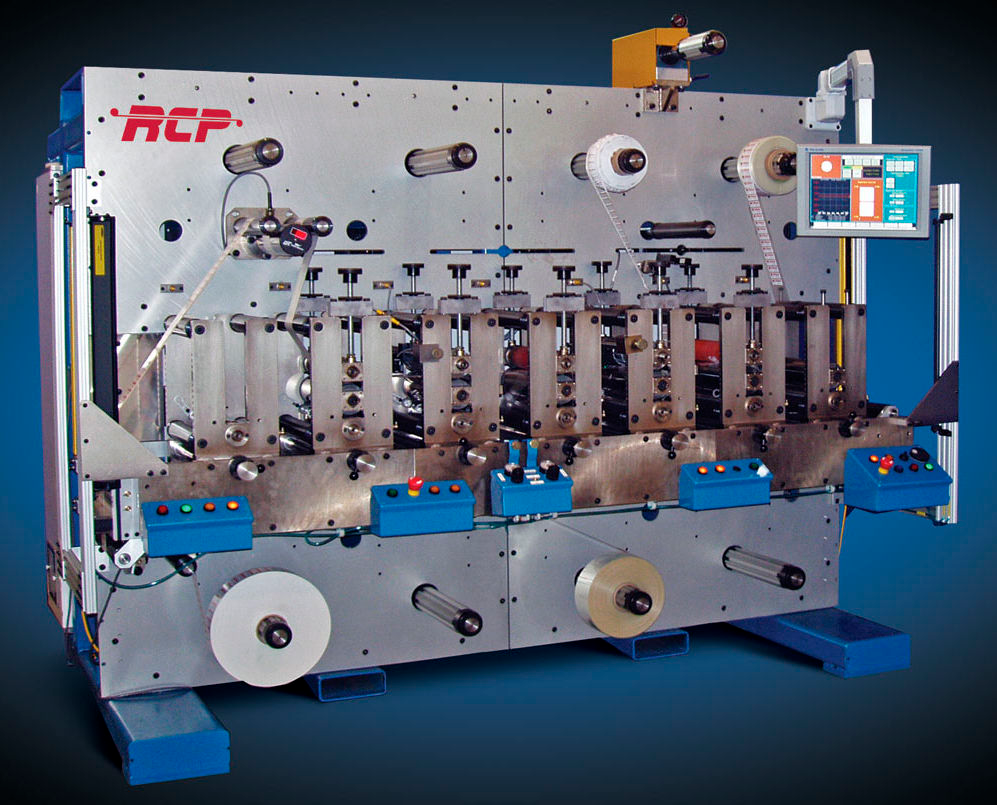
\includegraphics[height=3cm]{png/piece3}

\textit{Emporte pièce industriel (Machine à poinçonner, découper)}
\end{center}
\end{minipage}

\begin{contexte}
\begin{itemize}
\item Objectif pédagogique : représenter des éléments filetés dans un produit industriel
\item Objectif technique : concevoir les éléments filetés associés à un emporte pièce afin qu'il puisse remplir le cahier des charges
\end{itemize}
\end{contexte}

\subsection*{Fonction globale}
Le mécanisme étudié permet grâce à l’outil 6 de pratiquer une découpe fermée dans un matériau en feuille. La perforatrice de l'écolier est un emporte-pièce particulier.

\begin{center}
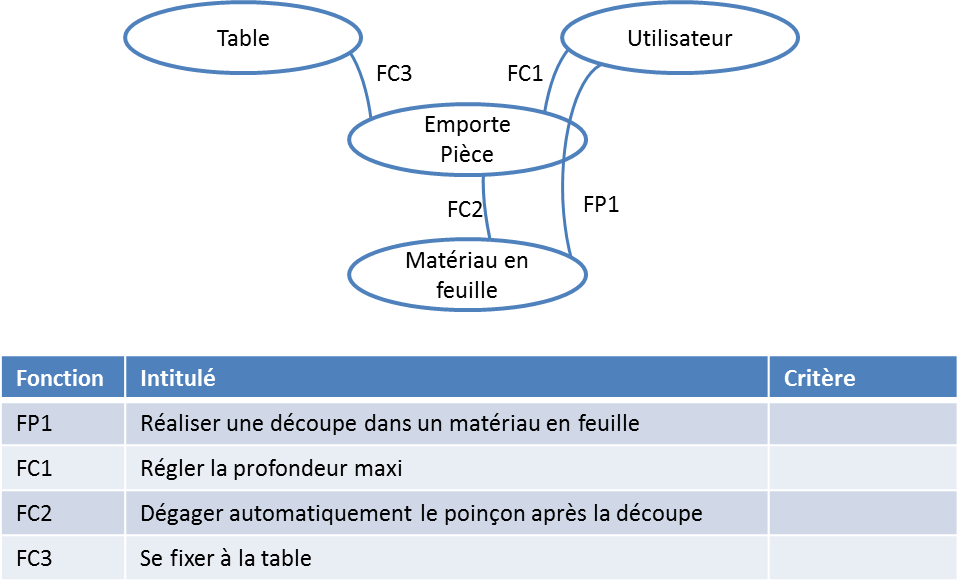
\includegraphics[width=12cm]{png/af}
\end{center}

\subsection*{Description du mécanisme}
Le dessin fourni représente à l’échelle 1 l’ébauche d’un mécanisme d’emporte-pièce en 3 vues incomplètes. Il est composé essentiellement :
\begin{itemize}
\item d'un bâti 1 en acier;
\item d'un levier de man\oe{}uvre 2 articulé autour de l’axe 4;
\item d'un ressort de rappel 3 non représenté;
\item d'un porte-outil 5 et de l’outil 6.
\end{itemize}

\subsection*{Travail à réaliser}
Toutes les modifications seront à porter simultanément sur toutes les vues. Seul le corps 1 sera dessiné avec la visserie demandée au 6\ieme point. 

\begin{enumerate}
\item Réalisation de FP1 : compléter la partie supérieure du bâti 1. Cette partie est entièrement usinée. Elle reçoit le levier 2 articulé autour de l'axe 4. Elle est arrondie à l'extrémité. On utilisera une coupe partielle.

\item Réalisation de FP1 : en A ajouter une nervure axiale d'épaisseur $e=8$ reliant la semelle de section carrée $80 \times 80$ au cylindre de section circulaire $\phi=34$, ce dernier recevant le porte-outil.

\item Réalisation de FC2 : en B prévoir un système d'accrochage pour la fixation du ressort 3.

\item Réalisation de FC3 : en C prévoir 4 trous pour vis $\phi 8$ pour fixation du bâti sur la table.

\item Réalisation de FP1 : en D prévoir deux bossages $\phi 32$.

\item Réalisation de FC1 : en E ajouter une vis $\phi 8$ servant de butée au levier 2 avec contre-écrou de blocage sur bossage $\phi 18$.
\end{enumerate}

\begin{center}
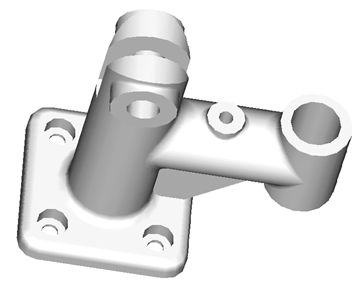
\includegraphics[width=.4\linewidth]{png/vue1}
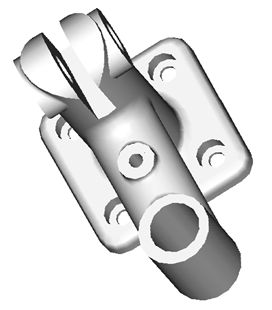
\includegraphics[width=.4\linewidth]{png/vue2}
\end{center}

\begin{center}
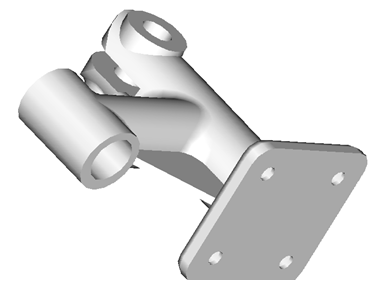
\includegraphics[width=.4\linewidth]{png/vue3}
\end{center}
\end{document}